\section{The two branching skeletons and a reduction}\label{sec:geometry}
Theorem~\ref{q3:thm:kernel} gives every tree with at most three branch vertices one orientation satisfying \eqref{eq:kernelbound} for every finite model, so it remains to treat $b(U)=4$.

Let $B$ be the four original branch vertices, and let $S$ be the minimal connected subtree of $U$ containing $B$. Every vertex of degree at least three in $S$ belongs to $B$, since it also has original degree at least three. Every leaf of $S$ belongs to $B$, by minimality. Suppressing the degree-two vertices of $S$ outside $B$ leaves a tree on exactly four vertices, which is either a path $P_4$ or a star $K_{1,3}$ (Figure~\ref{fig:skeletons}).

Each skeleton edge represents a positive-length path in the original tree, whose interior vertices have degree two and carry no side arms. Every component outside the core is a path attached at a branch vertex, since another branch point there would belong to $B$, contrary to the choice of $S$. These components are the \emph{side arms}, and the core paths together with the side arms partition the edges of $U$.

\begin{figure}[htbp]\centering
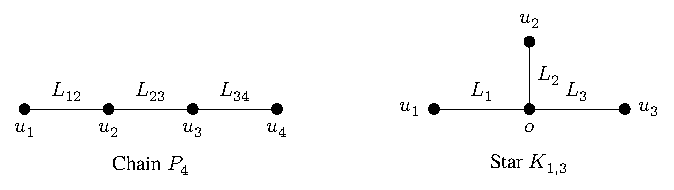
\includegraphics{figures/skeletons.pdf}
\caption{The two skeletons on four branch vertices. Each edge represents its original positive-length connector; side arms are omitted from the drawing.}\label{fig:skeletons}
\end{figure}

A leaf of the skeleton is called a \emph{terminal}. It has at least two actual side arms in $U$. Maximally pair its equal-length arms using \eqref{q3:eq:equalpair}.

\begin{lemma}[Reducible terminal]\label{lem:reduction}
If a terminal has zero or one residual side arm after equal-length pairing, then $U$ has a fixed orientation satisfying \eqref{eq:kernelbound}.
\end{lemma}
\begin{proof}
Orient the equal pairs so that their product is $E_i\le1$. Removing those paired arms for the comparison leaves the terminal vertex, its remaining arm if any, and all core edges; the terminal then has degree at most two and no other degree has increased. The comparison tree is nonempty, has at most three branch vertices, and carries a fixed orientation from Theorem~\ref{q3:thm:kernel}. Restoring those arms multiplies the nonnegative integrand at the terminal label by $E_i\le1$, preserving the density bound.
\end{proof}

The reduction applies to both skeletons. We may therefore assume that every terminal has at least two distinct residual lengths. Singleton internal side tables and singleton star-center tables survive the reduction and are estimated in Sections~\ref{sec:chain} and~\ref{sec:star}.
